\documentclass[14pt]{article}
\usepackage{graphicx}

\usepackage{multirow}
\usepackage{verse}
\newcommand{\attrib}[1]{%
\nopagebreak{\raggedleft\footnotesize #1\par}}
\renewcommand{\poemtitlefont}{\normalfont\large\itshape\centering}
 
\usepackage{chemfig}
\usepackage{circuitikz}
\usepackage{amsmath}

\usepackage{pgfplots}
\pgfplotsset{width=7cm,compat=1.8}

\usepackage{geometry}

\usepackage[%
  newcommands     % \RaggedRight=\raggedright etc. 
 ,newparameters   % use default settings of ragged2e
]{ragged2e}
\usepackage[pdfauthor={Sina Ahmadi},
            pdftitle={Using XeLaTeX for Kurdish}]{hyperref}
            
\hypersetup{colorlinks,breaklinks,
            urlcolor=[rgb]{0,0.5,0.5},
            linkcolor=[rgb]{0,0.5,0.5}}
            
            
\usepackage{listings}
\lstset{%
language={[LaTeX]TeX},
numbersep=5mm,
basicstyle=\footnotesize,
numbers=left,
stepnumber=1,
numberstyle=\tiny,
breaklines=true,frame=single,framexleftmargin=2mm, xleftmargin=2mm,
prebreak = \raisebox{0ex}[0ex][0ex]{\ensuremath{\hookleftarrow}},
backgroundcolor=\color{green!5},frameround=fttt,escapeinside=??,
rulecolor=\color{red},
morekeywords={
    maketitle},
keywordstyle=\color[rgb]{0,0,1},                    
        commentstyle=\color[rgb]{0.133,0.545,0.133},
        stringstyle=\color[rgb]{0.627,0.126,0.941}
%columns=fullflexible
}
% numerals: eastern and western

\usepackage{polyglossia}
\setdefaultlanguage[variant=Sorani,script=Latin,numerals=western]{kurdish} 
\setmainfont{Times New Roman}
\newfontfamily\arabicfont[Script=Arabic,Scale=1]{Yas}
\newfontfamily\greekfont{Times New Roman}[Script=Greek]
\let\arabicfonttt\ttfamily
\setotherlanguage{english}
\setotherlanguage[variant=poly]{greek}
\newfontfamily\kurdishfont[Script=Arabic,Scale=1,Ligatures=Contextual]{Yas}


\title{\textenglish{\XeLaTeX} bo Nûsînî Kurdî}
\author{Sîna Ehmedî \\ {\small \url{https://sinaahmadi.github.io/}}}
\date{\today}

\begin{document}

\maketitle
\tableofcontents

\begin{abstract}

Maweyek bû xulyay ewem hebû ke bitwanim \TeX bo nûsînî kurdî be kar bênim. Her ewe hanî dam ke xom Kurdî lê zyad bikem. Lem bełgeyeda bas le bekar hênanî \XeLaTeX legeł pekeycî \texttt{Polyglossia} bo nûsînî kurdî dekem. Le dwayîn weşanî kurdî lem pekeyceda, dû zarawey Soranî û Kirmancî be her dû řênûsî Latîn û Ërebî dabîn kirawin. Diłnyam eger be başî fêrî \TeX bin, dezanin çêjêk ke le be kar hênanî \TeX da heye le çi bernamey dîkeda nîye!

\end{abstract}


\section{\TeX~çî ye?}

\TeX sîstemêkî amade kirdnî bełge ye ke têyda nûser le deqî sakar legeł nîşanegelî taybetî bo nûsîn kełk werdegirê. Em boçûne cyawaz e le şêwazî dîkey dest werdanî deq ke têyda her şitêk bête çaw her ew şite ye ke çap debê û wekû akamî bełgeke nîşan dedirê. Boyeş be îngilîsî bem şêwaze dełên \textit{what you see is what you get}, yan be kurtî \textsc{WYSIWYG}. Microsoft Word nimûneyekî nasraw e ke lem şêwaze kełk werdegirê.

\TeX bo yekem car le sałî 1978 le layenî zana û bilîmetî kompyûter Donald Knuth ewe saz kira. \TeX le ser ew boçûneda pêkhatûwe ke nûser debê karî nûsîn bika nek řazandnewey deq. Wate, bo nûserî bełgeyek debê ew amêrane dabîn kirabê ke bitwanê be hemû pêdawîstîyekanî le nûsînda biga, bigre bo nûsînî firmûłêkî bîrkarî bê yan hawkêşeyekî kîmyayî yan parçe şîërêk. Boyeş, le nêw akadîmya û ew kesane ke be lêhatûyî le ser babetêkî zansitî denûsin le \TeX zor be berbiławî kełk werdegîrdirê. Wişey \TeX le wişey Yonanî \textgreek{\textit{τέχνη}}yewe dê ke be manay huner e. Le ber ewey fonîmî \textgreek{χ} le Kurdî û zor zimanda beranberêkî nîye, detwanîn le kurdî błeyn \textit{têk} yan \textit{têx}.

\paragraph{Taybetmendîyekanî \TeX}
Be kurtî, le taybetîmendîye here girîngekanî têk emane in:
 
\begin{itemize}
\item nûsînî govar, kitêb, řaportî teknîkî û siłaydî amadekarî
\item beřêwe birdinî bełge gewrekan ke zor beş û bend û serçaweyan têda ye
\item nûsînewey firmûłe piř wirdekarîyekan le bîrkarîda
\item saz kirdinî otomatîkî serçawekan
\item be asanî kełk wergirtin le wêne û dyagram
\item gořanewe be şêwekanî dîkey nîşan danî deq wekû HTML
\end{itemize}

Her le ser binemay \TeX ewe, diwatir çendîn berhemî dîke dabîn kiran ke têyanda taybetmendîgelî zortir ře çaw degîrdirê, wekû nûsîn be zimananî dîke û be řênûsî cyawaz le řênûsî Latîn. \LaTeX~ û \XeLaTeX~ dû nimûney benêwbang in ke be taybet lem serdemeda kełkyan lê werdegîrdirê.


\section{Çon \TeX~be kar bênim?}

Bo kełk wergirtin le \TeX le ser kompyûtereket le pêş hemû şitêk debê bernameket damezrandibê. Bełgeyekî sakar le \TeX da le wêney \ref{fig_mwe} nîşan dirawe.

\begin{figure}[h]
    \centering
        \begin{minipage}{0.65\textwidth}
\begin{lstlisting}
\documentclass{article}
\usepackage[utf8]{inputenc}

\title{An Example}
\author{Sina Ahmadi}
\date{\today}

\begin{document}

\maketitle
\section{Introduction}

This is a minimal working example in \LaTeX.

\section{Conclusion}

The joy of writing Kurdish in \TeX.

\end{document}

\end{lstlisting}
    \end{minipage}\hfill
    \begin{minipage}{0.29\textwidth}
        \fbox{
               \centering
        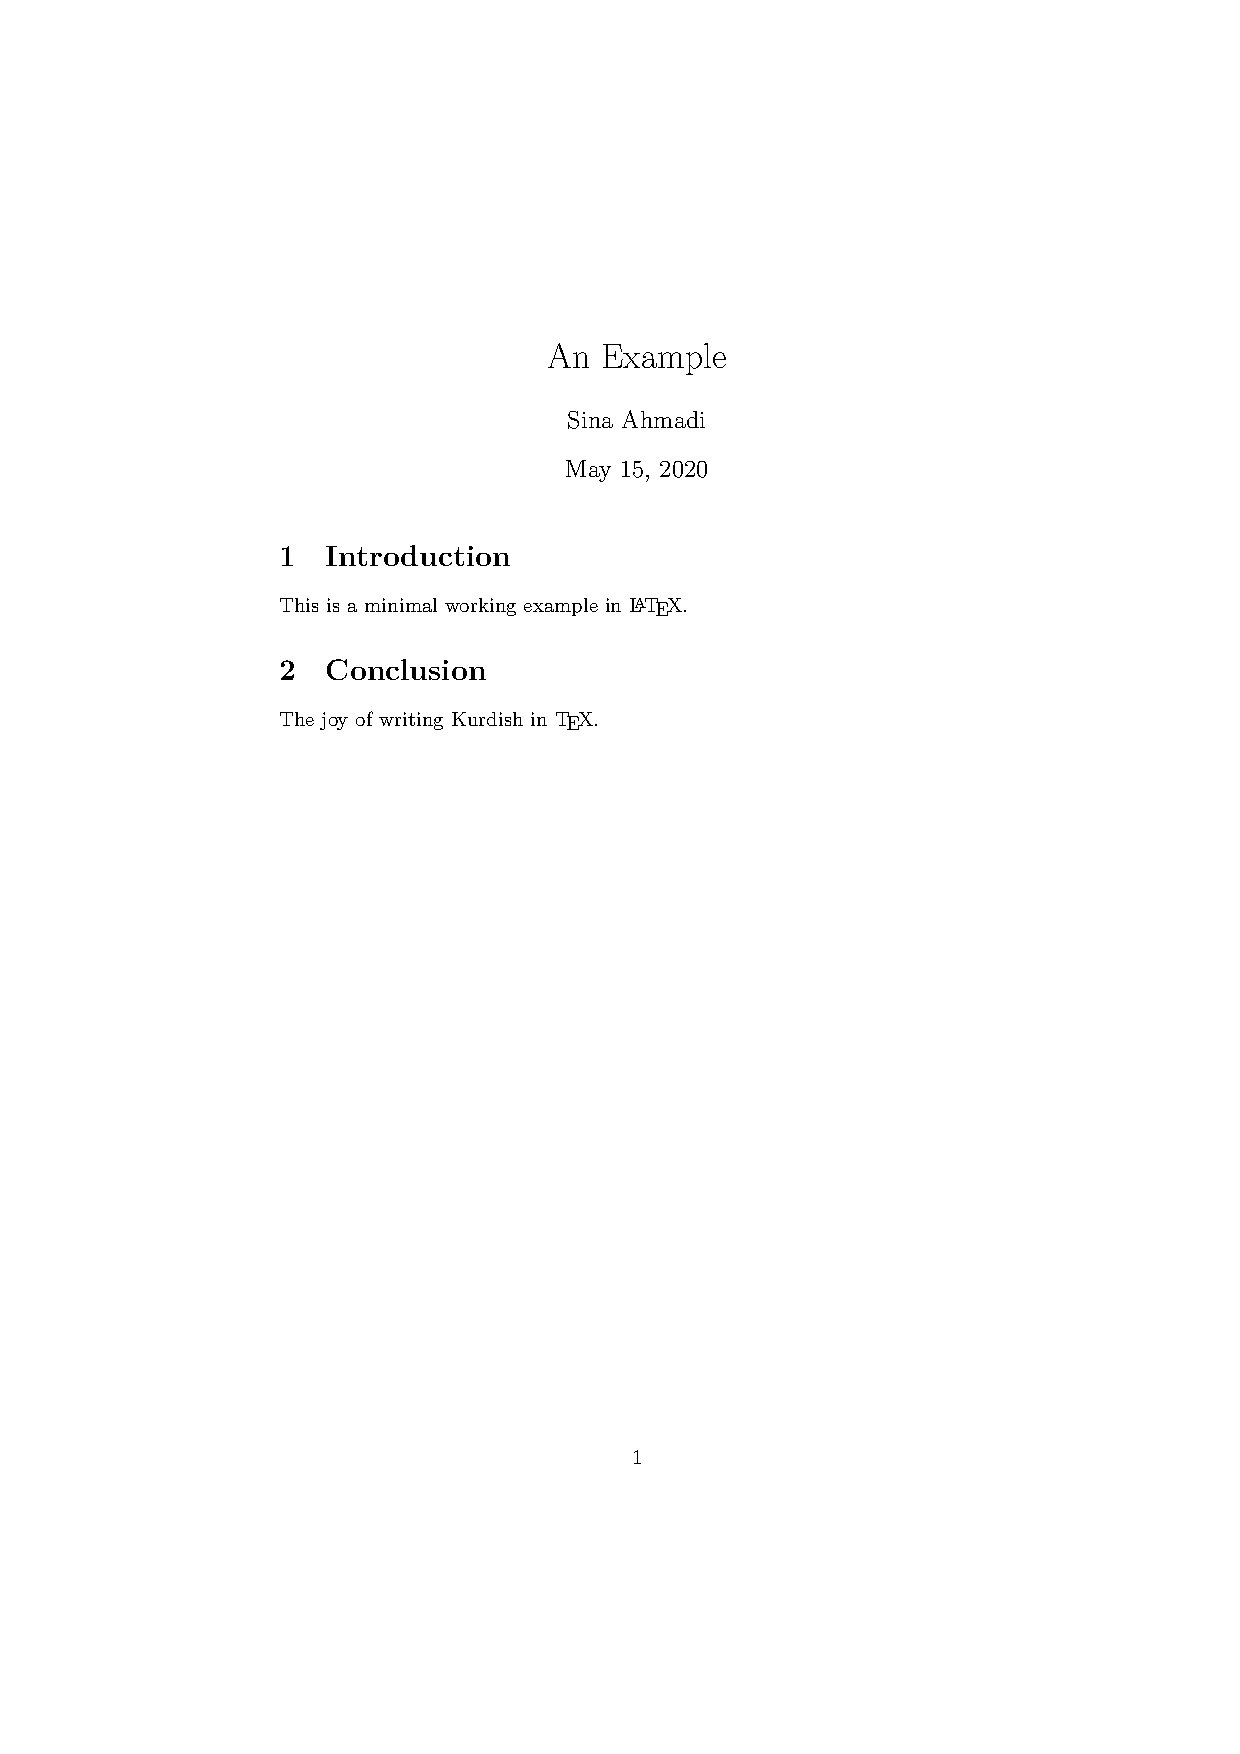
\includegraphics[width=\textwidth]{figure_example.pdf} 
        }
    \end{minipage}
 \caption{Nimûneyek le bełgeyek ke be \LaTeX~ nûsrawe. Le lay çepewe, kodî bełgekeye û le lay řastîşewe akamî kampayl kirdinyetî}
 \label{fig_mwe}
\end{figure}


Êste pirsyar ewe ye aya her em şêweyeş detwanîn bo nûsînî kurdî be kar bênîn? Serinc den ke lew nimûneyeda le wêney \ref{fig_mwe} ke le serê dîtman, ne mêjû, ne jimarey beşekan û ne tenanet ewey ke babeteke le kwêy bełgekeda bê û qebarey lapeřeke çon bê be ême cêbecê nekirawe. Wate, \TeX~ bo xoy bełgekeman be hemû ew wirdekarîyanewe saz deka. Ca bo ye, ew kesaney ke çêjî kar kirdin be têk deçêjin, qet natwanin bgeřênewe ser sîstimanî pêkhênanî deq (typesetting) î dîke wekû Microsoft Office! Bo ewey zortir legeł pêkhatekanî bełgekan le \TeX~ aşina bin çaw le \cite{wilkins1995getting} biken.



\section{\XeLaTeX~bo nûsînî Kurdî}

Kêşeyek ke pêştir le be kar hênanî \TeX~ da hebû, be kar hênanî zimanan û řênûsanî dîke bû. \XeLaTeX sîstimêke ke le ser \TeX~ ewe saz kirawe û biřyar wa ye ke le Unicode bo nûsînî hemû zimanêk kełk wergirê. Bo ye be xoşhałîyewe detwanîn le cwanîy sîstimî pêkhênanî deqî \TeX bo nûsînî Kurdî kełk wergirîn.

\texttt{Polyglossia}\footnote{\url{https://github.com/reutenauer/polyglossia}}  pekeycêk e ke bo be kar hênanî zimane corawcorekan le \XeLaTeX~ saz kirawe. Zimanî Kurdî çendîn zarawe û řênûsî heye. Lem doxeda, dû zaraweman lew pekeyce bo Kurdî zyad kirdûwe: Soranî û Kirmancî. Bo her dû zarawekeş, dû řênûsî Latîn û Ërebî dabîn kirawe. Wate, eger bełgeyek Soranî bê, be her dû řênûseke detwanin binûsin, bo Kirmancîş her bew şêweye. Bo be kar hênanî Kurdî, bełgeketan debê bem şêweye bê:

\begin{lstlisting}
 \documentclass{article}
 \usepackage{polyglossia}

 \setdefaultlanguage[variant=sorani,script=Arabic,numerals=eastern]{kurdish}
 \newfontfamily\arabicfont[Script=Arabic,Scale=1]{Yas}
 \let\arabicfonttt\ttfamily

 \begin{document}
 \end{documentu}
\end{lstlisting}

Debê bełgeketan bew hełbijardane pêk bênin ke le hêłî 4da dyarî kirawe ke lêyda zarawe, řênûs û şêwey jimarekan dyarî deken. Xiştey ~\ref{tab_polyglot_options} sercem hełbijardekan nîşan deda ke le dwayîn weşanî Kurdî le ser \texttt{Polyglossia}da heye.

\begin{table}[h]
\centering
\begin{tabular}{l|l|l|l} 
 \hline
Polyglossia         & variant  & script        & numerals         \\ \hline \hline
\multirow{2}{*}{Kurdish} & \texttt{sorani}   & \texttt{arabic}, \texttt{latin} & \texttt{eastern}, \texttt{western} \\  \cline{2-4} 
                         & \texttt{kurmanji} & \texttt{arabic}, \texttt{latin} & \texttt{eastern}, \texttt{western} \\ \hline
\end{tabular}
\caption{hełbijardekan bo pêk hênanî bełgeyek be Kurdî le \texttt{Polyglossia}}
\label{tab_polyglot_options}
\end{table}


Kewa bû, bo nimûne, eger bitanhewê bełgeyek be Kirmancî binûsin û le řênûsî Latîn kełk wergrin, detwanin hêłî 4 bem şêweye bigořin:

\begin{english}
\begin{lstlisting}
 \setdefaultlanguage[variant=kurmanji,script=latin,numerals=western]{kurdish}
\end{lstlisting}
\end{english}

Le weşanî êstada, tenya řojjimêrî zayînî detwanê be kar bihêndirê. Nêwî mangekan bew şêweyeye ke le xiştey \ref{tab_polyglot_calendar}da nîşan dirawe. Cêgay serinc e ke dû şêwaz hen bo nîşan danî mêjû: \texttt{\textbackslash today} û \texttt{\textbackslash ontoday}. Le şêwazî yekemda, tenya nêwî mangeke û jmarey řoj û sał dên. Le şêwazî dwayînda, le nêwan sê beşeke "î/y"î îzafe dandendirê.


\begin{table}[h]
\centering
\begin{tabular}{|l|l|l|l|l|} 
\hline
Îngilîsî & Sorani-Ërebî & Sorani-Latin & Kurmancî-Ërebî & Kurmancî-Latin \\\hline\hline
January & {\kurdishfont{ دووهەم كانوونی}} & Kanûnî Dûhem  & {\kurdishfont{پاشین  چلەیا}} & Çileya Paşîn \\ 
February & {\kurdishfont{شوبات}} & Şubat & {\kurdishfont{شبات }} & Sibat \\
March & {\kurdishfont{ ئازار }} & Azar & {\kurdishfont{ ئادار }} & Adar \\
April & {\kurdishfont{نیسان }} & Nîsan & {\kurdishfont{ نیسان }} & Nîsan \\
May & {\kurdishfont{ئایار }} & Ayar & {\kurdishfont{ گولان }} & Gulan \\
June & {\kurdishfont{حوزەیران }} & Huzeyran & {\kurdishfont{ حەزیران }} & Hezîran \\
July & {\kurdishfont{ تەممووز }} & Temmûz & {\kurdishfont{ تیرمەهـ }} & Tîrmeh \\
August & {\kurdishfont{ ئاب }} & Ab & {\kurdishfont{ تەباخ }} & Tebax \\
September & {\kurdishfont{ئەیلوول }} & Eylûl & {\kurdishfont{ ئیلۆن }} & Îlon \\
October & {\kurdishfont{  یەكەم تشرینی}} & Tişrînî Yekem & {\kurdishfont{  پێشین چریا  }} & Çiriya Pêşîn \\
November & {\kurdishfont{  دووهەم تشرینی}} & Tişrînî Dûhem & {\kurdishfont{ پاشین چریا }} & Çiriya Paşîn \\
December & {\kurdishfont{  یەكەم كانوونی}} & Kanûnî Yekem & {\kurdishfont{پێشین چلەیا  }} & Çileya Pêşîn \\ \hline
\end{tabular}
\caption{Name of the months in the Kurdish calendars in \texttt{Polyglossia}}
\label{tab_polyglot_calendar}
\end{table}


Bo zanyarî zyatir sebaret be \texttt{Polyglossia} û zimanî Kurdî lem pekeyceda, çaw le  \cite{Charette2020} û \cite{ahmadi2020TexforKurdish} biken.

\newpage

\section{Çend nimûne be \texttt{Polyglossia} bo Kurdî}

\subsection{\XeLaTeX~ bo wêje û huner}

\poemtitle*{Yadigarî şîrîn}
\settowidth{\versewidth}{Çawekem! Çawî řeşî to afetî gyanî min e}
\begin{verse}[\versewidth]
çawekem! Çawî řeşî to afetî gyanî min e \\
gyanekem! Birjangî tîjit nûke řimbî dujmin e \\
\vin şîrî destî şêrî ała ye biro řakşaweket \\
\vin cergî lawêkî hejarî Kurdî wird pê bincine \\ 
çon debê serbest gelî jêrdest ke kiç dabeste bê? \\
bes nebê ew koyletî û ew kiç le jûr dabestine \\
\vin derkî daxistûwe le to babit keçî derkî nîye \\
\vin derke daxistin le to derkî humêd daxistine \\
\end{verse}
\attrib{Le dîwanî Mamosta Hêmin}

\subsection{\XeLaTeX~bo zanist û bîrkarî}

\begin{center}
\setchemfig{atom sep=2em,bond style={line width=1pt,red,dash pattern=on 2pt off 2pt}}  
\chemname
{\chemfig{H-C(-[2]H)(-[6]H)-C(=[1]O)-[7]H}}
{Êtanal (Ethanal)}
\end{center}


\begin{equation}\label{equation_example}
  x = a_0 + \frac{1}{\displaystyle a_1 
          + \frac{1}{\displaystyle a_2 
          + \frac{1}{\displaystyle a_3 + a_4}}}
\end{equation}


\begin{figure}
\centering
\begin{minipage}[b]{.48\textwidth}
% source of the following: https://www.overleaf.com/learn/latex/CircuiTikz_package
\begin{circuitikz}[american voltages]
\draw
  (0,0) to [short, *-] (6,0)
  to [V, l_=$\mathrm{j}{\omega}_m \underline{\psi}^s_R$] (6,2) 
  to [R, l_=$R_R$] (6,4) 
  to [short, i_=$\underline{i}^s_R$] (5,4) 
  (0,0) to [open, v^>=$\underline{u}^s_s$] (0,4) 
  to [short, *- ,i=$\underline{i}^s_s$] (1,4) 
  to [R, l=$R_s$] (3,4)
  to [L, l=$L_{\sigma}$] (5,4) 
  to [short, i_=$\underline{i}^s_M$] (5,3) 
  to [L, l_=$L_M$] (5,0); 
  \end{circuitikz}
\caption{Serkit bo nimûne}
\label{example_circuit}
\end{minipage}\hfill
\begin{minipage}[b]{.4\textwidth}
  \centering
\begin{tikzpicture}
\begin{axis}[
    title={$x \exp(-x^2-y^2)$}, 
    xlabel=$x$, ylabel=$y$,
	small,
]
\addplot3[
	surf,
	domain=-2:2,
	domain y=-1.3:1.3,
] 
	{exp(-x^2-y^2)*x};
\end{axis}
\end{tikzpicture}
\caption{Fanckşinêkî matmatîk}
\label{example_function}
\end{minipage}
\end{figure}


\section{Kotayî}

Lem nûsraweyeda be kurtî basî \TeX~ man kird û çonayetî be kar hênanî \XeLaTeX~ legeł pekeycî \texttt{Polyglossia} bo nûsînî Kurdîman xiste řû. Bo zanyarî zyatir sebaret be piřôjey \XeLaTeX~î Kurdî, serdanî małpeřî \url{http://kurdishtex.github.io} biken.



\bibliographystyle{unsrt}
\bibliography{bibliographylatin}

\end{document}
